% The section about the place of the simulation itself
% @author Kalvin Döge
%


\section{Simulationsort}\label{sec:simulationplace}

Für die Arbeit wurde die Binnen- und Außenalster als Simulationsumgebung ausgewählt.

\begin{figure}[h]
    \centering
    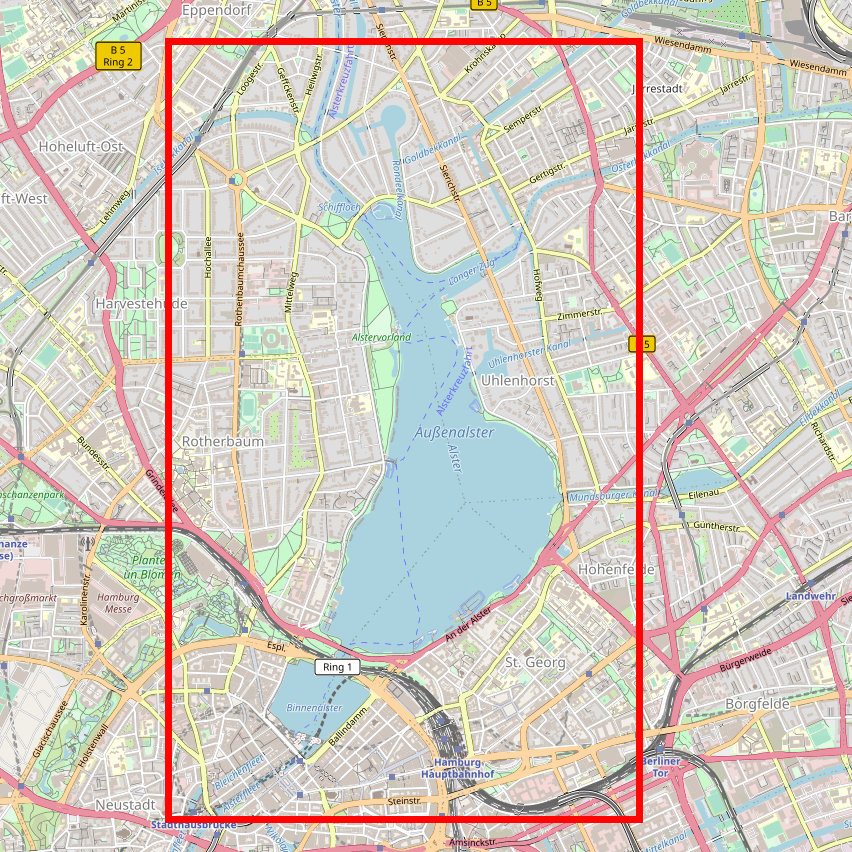
\includegraphics[width=0.75\textwidth]{sim-area}
    \caption{Simulationsumgebung}
    \label{fig:sim-area}
\end{figure}

Wie im Ausschnitt~\ref{fig:sim-area} zu erkennen ist, ist aufgrund der zentralen Lage innerhalb der Stadt, vieler anliegenden Kreuzungen und generell dichter Besiedelung um die Alster herum eine hohe Dichte an Agenten für die Simulation gegeben, die eine ,,Grüne Welle`` für Fahrradfahrer erschweren können.
Dies gibt der Simulation auf der einen Seite eine Herausforderung, mit schwereren Vorgaben überhaupt eine Lichtsignalschaltung für die ,,Grüne Welle`` zu finden, während auf der anderen Seite dafür aber diese Simulation wie eine ,,Obergrenze`` angesehen werden kann für die Agenten- und Lichtsignalanzahlen.
